% ------------------------------------------------------------------------------------
% ------------------------------ GESTION DE USUARIOS ---------------------------------
% ------------------------------------------------------------------------------------
\clearpage
\section{Gestión de Usuarios}

    Usted como Jefe de la División de  Innovación Académica podrá realizar la gestión sobre los siguientes usuarios:
    \begin{itemize}
        \item Analista.
        \item Jefe de Departamento de Desarrollo e Innovación Curricular
    \end{itemize}

    % ------------------------------------------------------------------------------------
    % ----------------------------- CONSULTA DE USUARIOS ---------------------------------
    % ------------------------------------------------------------------------------------

    \subsection{Consulta de Usuarios}
  Para poder ver la lista de usuarios que tiene a su cargo, primero debe seleccionar la opción \textbf{Gestionar Usuarios} del menú ubicado en la parte izquierda, así podrá observar la siguiente pantalla:

  % Imagen de Consultar usuarios
  \begin{figure}[H]
  	\centering
  	\hypertarget{consultarUs}{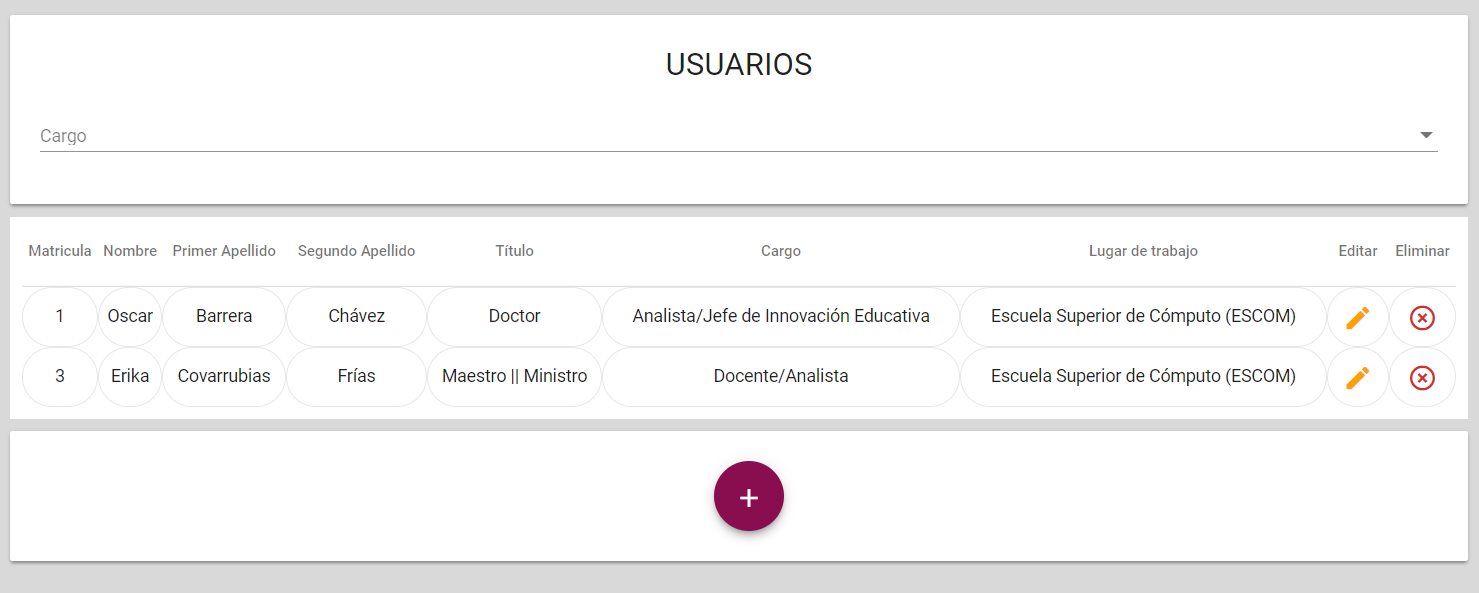
\includegraphics[width=0.6\linewidth]{images/SP5/Consultar-Usuario}}
  	\caption{Pantalla para consultar usuarios}
  	\label{consultarrh}
  \end{figure}

  En esa pantalla, aparecerán de forma predeterminada todos los usuarios que tiene a su cargo y que están registrados en el sistema hasta el momento. Tendrá a su disposición 2 funciones:
  
  \begin{enumerate}

  	\item   Buscar usuarios según el cargo que ocupan.

  	Para esto solo tendrá que seleccionar el cargo que desea consultar en el siguiente componente:

  	\begin{figure}[H]
  		\centering
  		\hypertarget{cargo1}{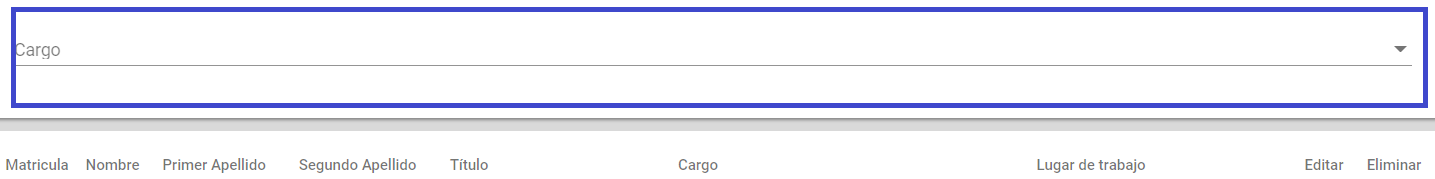
\includegraphics[width=0.7\linewidth]{images/SP5/BtnCargo1}}
  		\caption{Selección de Cargo}
  		\label{cargo1}
  	\end{figure}

  	Y a continuación el sistema mostrará todos los usuarios que tengan el cargo seleccionado.

  	   \newpage

  	\item Eliminar usuarios.

  	Para esta última acción, usted solo deberá dar clic en el botón con el icono de una equis en color rojo que está al lado del usuario que desee  eliminar.

  	\begin{figure}[H]
  		\centering
  		\hypertarget{eliminar}{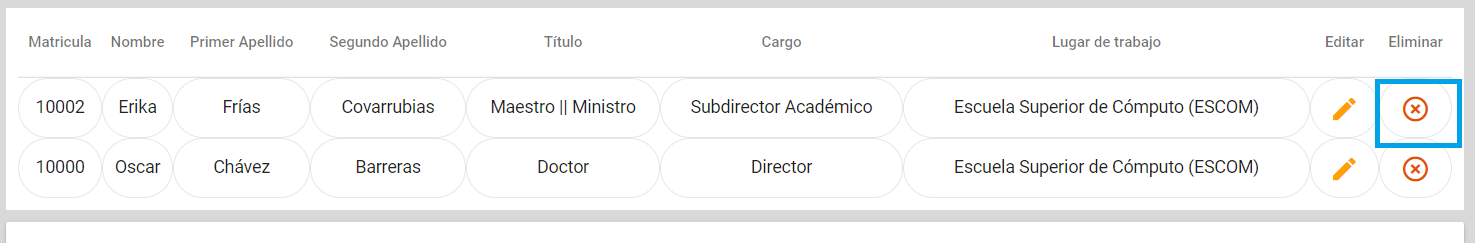
\includegraphics[width=0.7\linewidth]{images/SP5/BtnEliminar}}
  		\caption{Botón Eliminar Usuarios}
  		\label{eliminar}
  	\end{figure}

  	Al hacer esto, el sistema desplegará el siguiente mensaje:

  	%Imagen del MSG22
  	\begin{figure}[H]
  		\centering
  		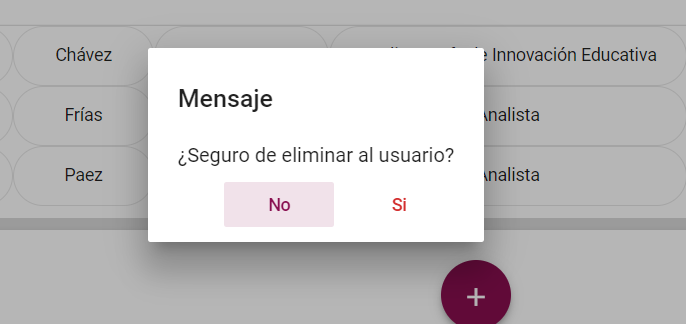
\includegraphics[width=0.4\linewidth]{images/SP5/MSG22}
  		\caption{Confirmación de eliminación}
  		\label{confirmarE}

  	\end{figure}

  	Para confirmar, usted deberá dar clic en el botón “Sí”, y en ese momento el usuario será removido del sistema y usted permanecerá en la pantalla \hyperlink{consultarUs}{\textit{Consultar Usuarios}}.
  	Para cancelar, usted deberá dar clic en botón “No”, y en ese momento el mensaje se cerrará, el usuario no se eliminará, y usted permanecerá en la pantalla de \hyperlink{consultarUs}{\textit{Consultar Usuarios}}.

  \end{enumerate}

  También mediante botones de esta pantalla podrá acceder a las siguientes 2 funciones:

  \subsubsection{Editar usuarios}

  Para esto, usted solo deberá dar clic en el botón con el icono de un lápiz amarillo que está al lado del usuario que desea modificar. Al hacer esto el sistema le mostrará la pantalla   de \hyperlink{editarUs}{\textit{Editar Usuario}}.

  \begin{figure}[H]
  	\centering
  	\hypertarget{editar}{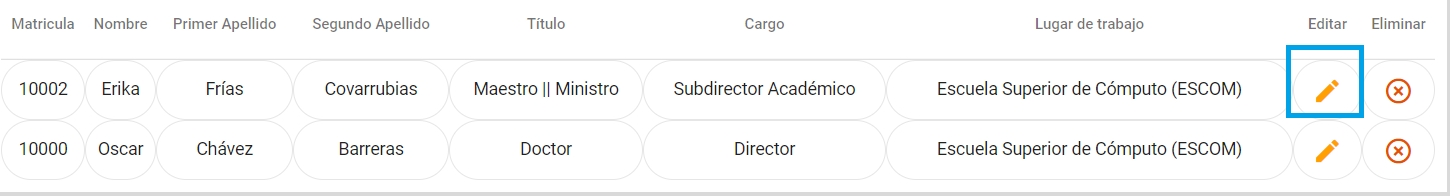
\includegraphics[width=0.7\linewidth]{images/SP5/BtnEditar}}
  	\caption{Botón Editar Usuarios}
  	\label{editar}
  \end{figure}

  Para más detalles de editar usuarios vaya a la sección \hyperlink{editar-user}{Edición de Usuarios}.

  \subsubsection{Registrar  usuarios}

  Para esto solo tendrá que dar clic en el botón “+” en la parte inferior de la pantalla. Al hacerlo, el sistema  lo redireccionará a la pantalla de \hyperlink{registrarUs}{\textit{Registrar Usuario}}.

  \begin{figure}[H]
  	\centering
  	\hypertarget{add}{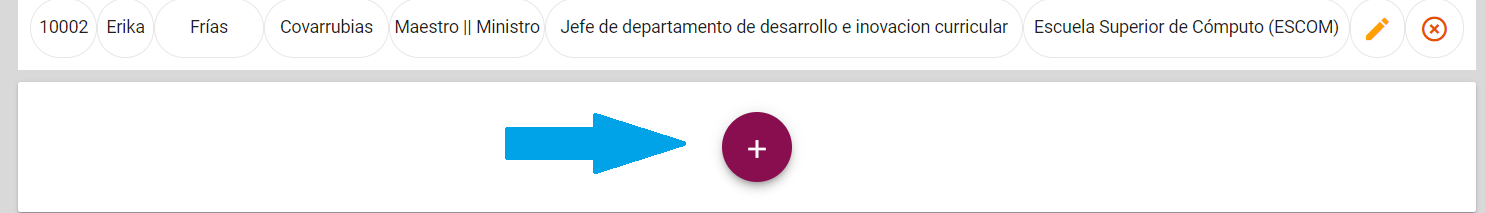
\includegraphics[width=0.7\linewidth]{images/SP5/BtnAgregar}}
  	\caption{Botón Agregar Usuarios}
  	\label{add}
  \end{figure}

  Para más detalles de registrar usuarios vaya a la sección \hyperlink{registrar-Us}{Registrar usuario}.

  \subsubsection{Posibles errores}
  \begin{itemize}
  	\item Si al  presionar la opción Gestionar Usuarios no se carga la información de los cargos disponibles para usted se presentará el siguiente mensaje:

  	% Imagen del MSG7
  	\begin{figure}[H]
  		\centering
  		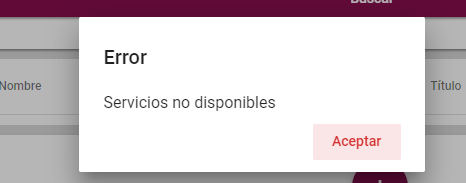
\includegraphics[width=0.4\linewidth]{images/SP5/MSGSN}
  		\caption{Servicios no disponibles}
  		\label{SND}

  	\end{figure}

  	Al dar clic en en botón ''Aceptar'', el sistema continuará en la pantalla  \hyperlink{consultarUs}{\textit{Consultar Usuarios}} y tendrá que intentarlo  mas tarde.

  	\item Si al consultar usuarios no se encuentra ninguno con el cargo solicitado se presentará el siguiente mensaje:
  	% Imagen del MSG21
  	\begin{figure}[H]
  		\centering
  		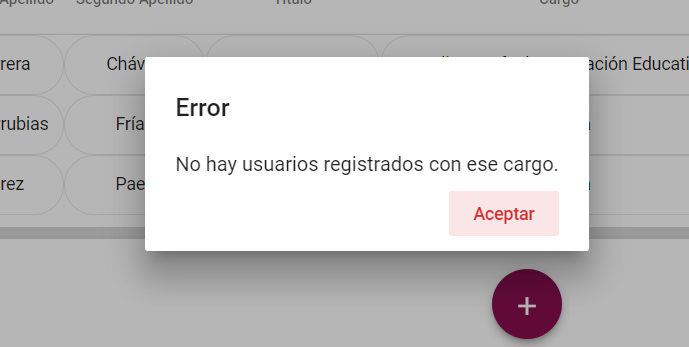
\includegraphics[width=0.4\linewidth]{images/SP5/MSG21}
  		\caption{No hay usuarios con ese cargo}
  		\label{mensaje21}
  	\end{figure}

  \end{itemize}


  % ------------------------------------------------------------------------------------
  % ----------------------------- REGISTRAR  USUARIOS ---------------------------------
  % ------------------------------------------------------------------------------------

  \newpage
  \hypertarget{registrarUs}{}
  \subsection{Registrar Usuarios}
  Si usted  en la pantalla de \hyperlink{consultarUs}{\textit{Consultar Usuarios}} dio clic en el botón ''+'', aparece la siguiente pantalla:

  \begin{figure}[H]
  	\centering
  	\hypertarget{registrar-Us}{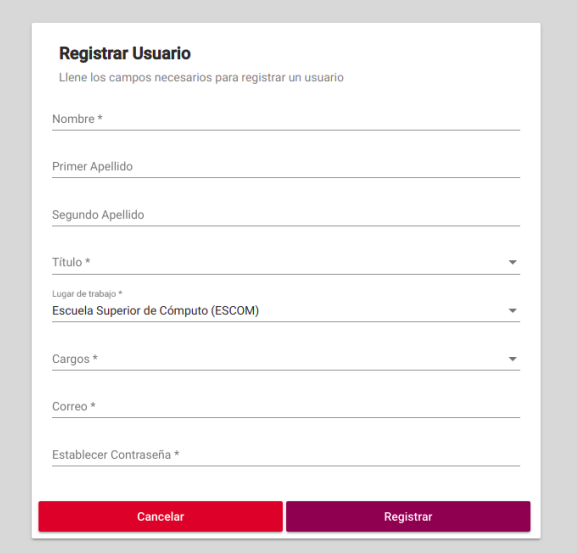
\includegraphics[width=0.7\linewidth]{images/SP5/Registro-Usuario-vacio}}
  	\caption{Pantalla para registrar usuarios}
  	\label{registrarrh}
  \end{figure}

  Usted tendrá que ingresar la información correspondiente del nuevo usuario en el formulario. Un ejemplo del llenado  sería el siguiente:

  \begin{figure}[H]
  	\centering
  	\hypertarget{ejreg}{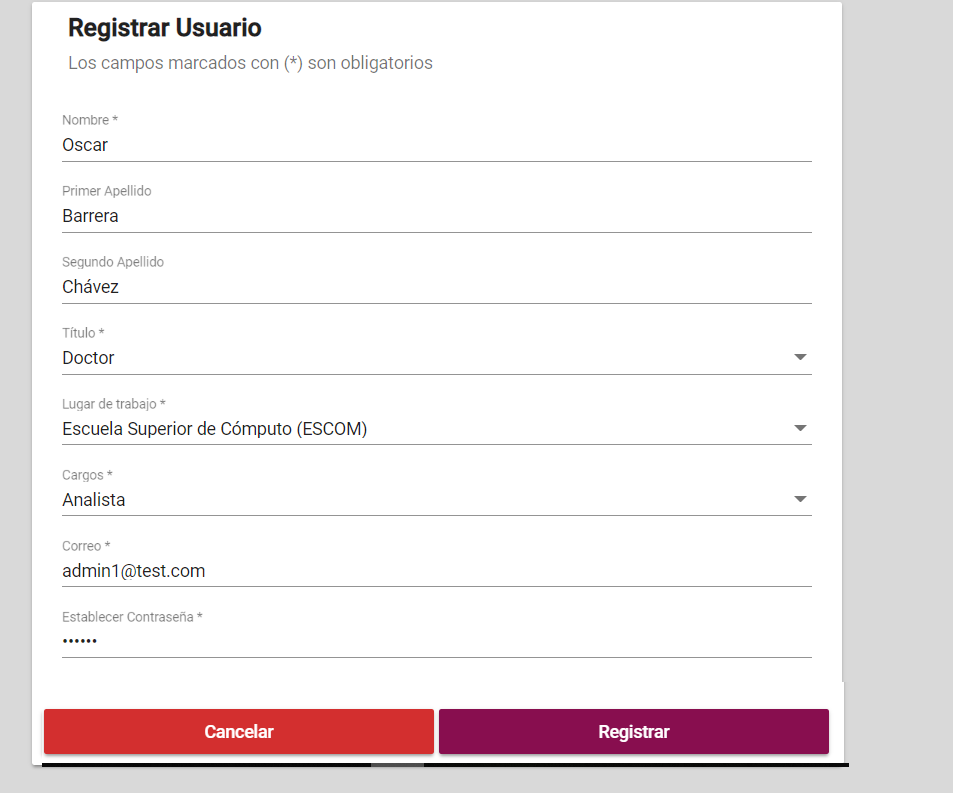
\includegraphics[width=0.7\linewidth]{images/SP5/Registro-Usuario-UA}}
  	\caption{Ejemplo de llenado para agregar un nuevo Usuario}
  	\label{ejreg}
  \end{figure}

  \newpage
  Si usted presiona el botón de “Cancelar”:

  \begin{figure}[H]
  	\centering
  	\hypertarget{cancel1}{
\includegraphics[width=0.7\linewidth]{images/SP5/BtnCancelar1}}
  	\caption{Botón ''Cancelar''}
  	\label{cancel1}
  \end{figure}

  El sistema mostrará el siguiente mensaje:

  %Imagen MSG29

  \begin{figure}[H]
  	\centering
  	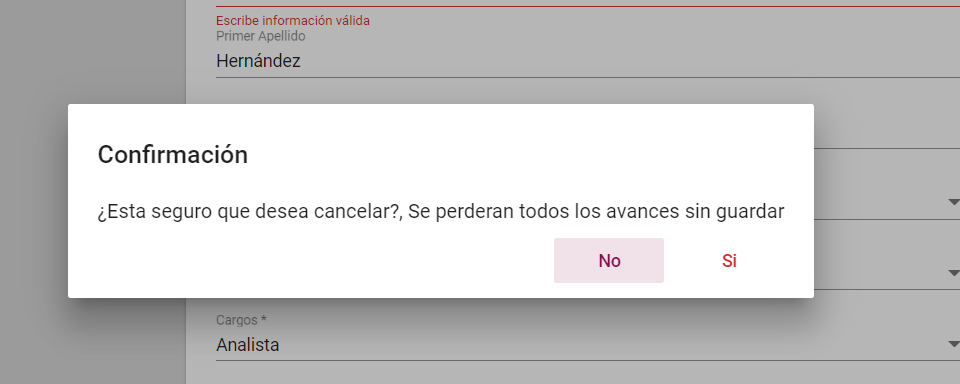
\includegraphics[width=0.4\linewidth]{images/SP5/MSG29}
  	\caption{Cancelar Accion}
  	\label{mensaje29}
  \end{figure}

  Para confirmar, usted tendrá que dar clic en el botón “Sí”, el usuario no será registrado y regresará a la pantalla de \hyperlink{consultarUs}{\textit{Consultar Usuarios}}.

  Para continuar con el registro, usted tendrá que  dar clic el botón “No”, el mensaje se  cerrará y usted continuará en el formulario para terminar el registro.

  Cuando usted considere que los datos son correctos y están completos, deberá de dar clic en el botón “Registrar”.

  \begin{figure}[H]
  	\centering
  	\hypertarget{btnreg}{
\includegraphics[width=0.7\linewidth]{images/SP5/BtnRegistrar}}
  	\caption{Botón ''Registrar''}
  	\label{btnreg}
  \end{figure}

  Si no se presentan errores el sistema muestra el mensaje:

  % Imagen MSG5

  \begin{figure}[H]
  	\centering
  	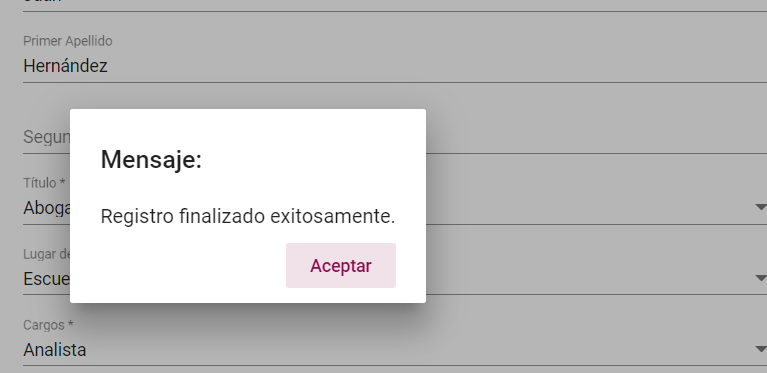
\includegraphics[width=0.4\linewidth]{images/SP5/MSG5}
  	\caption{Registro exitoso}
  	\label{mensaje5}

  \end{figure}

  Al dar clic en el botón “Aceptar”, el sistema mostrará la pantalla de  \hyperlink{consultarUs}{\textit{Consultar Usuarios}}.

  \subsubsection{Posibles errores}

  \begin{itemize}
  	\item Problemas con la conexión o el sistema

  	Si al momento de acceder a la pantalla de \hyperlink{registrarUs}{\textit{Registrar Usuario}} o al intentar registrar un usuario , aparece el siguiente mensaje:
  	%Imagen MSG7 Y MSG25

  	\begin{figure}[H]
  		\centering
  		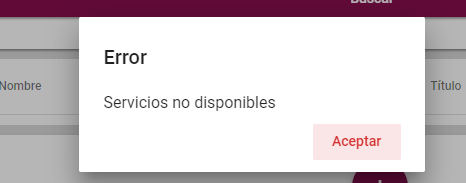
\includegraphics[width=0.4\linewidth]{images/SP5/MSGSN}
  		\caption{Servicios no disponibles}
  		\label{SND}

  	\end{figure}

  	Significa que existió un error de conexión o del sistema. Al dar clic en en botón ''Aceptar'', el sistema lo redireccionará a la pantalla de \hyperlink{consultarUs}{\textit{Consultar Usuarios}}. Deberá esperar a que la página este disponible para  intentar acceder nuevamente.

  	\item Campos vacíos al momento de agregar un nuevo usuario

  	Si usted deja en blanco algún campo o campos del formulario, y posteriormente dio clic en el botón ''Registrar'', el sistema mostrará el siguiente mensaje debajo del campo o campos :
  	%Imagen MSG44

  	\begin{figure}[H]
  		\centering
  		
\includegraphics[width=0.4\linewidth]{images/SP5/MSG44}
  		\caption{Campos vacíos}
  		\label{mensaje44}
  	\end{figure}

  	Regresará al formulario, en donde usted deberá llenar el o los campos que dejo vacíos.

  	\item El correo ingresado ya existe

  	Si al momento de dar clic en el botón ''Registrar'' aparece el siguiente mensaje:
  	%Imagen MSG36

  	\begin{figure}[H]
  		\centering
  		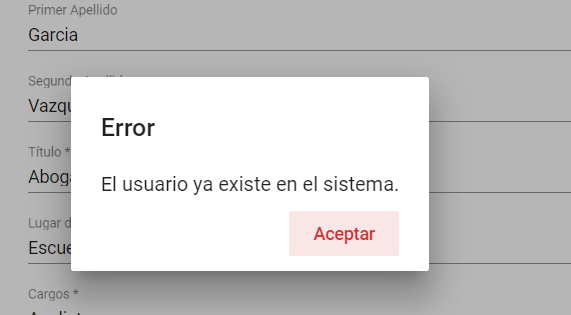
\includegraphics[width=0.4\linewidth]{images/SP5/MSG36}
  		\caption{El usuario ya existe}
  		\label{mensaje36}

  	\end{figure}

  	Significa que el usuario ya se encuentra registrado en el sistema, por lo que éste impide que se vuelva a agregar nuevamente. Al dar clic en botón ''Aceptar'', el mensaje se cerrará y usted  regresará al formulario. Aquí usted puede hacer dos acciones: verificar que el correo sea uno no registrado previamente e intentar agregar al usuario nuevamente, o abandonar la pantalla de \hyperlink{registrarUs}{\textit{Registrar Usuarios}} e ir a otras partes del sistema.
  	\newpage
  	\item Los campos ingresados no son válidos

  	Si al momento de dar clic en el botón ''Registrar'' aparece el siguiente mensaje:
  	%Imagen MSG35
  	% Imagen del MSG35
  	\begin{figure}[H]
  		\centering
  		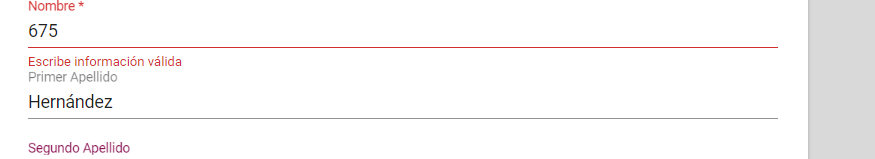
\includegraphics[width=0.4\linewidth]{images/SP5/MSG35}
  		\caption{Campos incorrectos}
  		\label{mensaje35}

  	\end{figure}

  	Significa que la composición de los datos ingresados en el formulario no es la correcta. Tenga en cuenta lo siguiente:

  	\begin{itemize}
  		\item El nombre y apellidos debe iniciar con mayúscula, puede poner más de uno por campo en caso de 2 nombres o apellidos compuestos.
  		\item Usted alteró la información de los selectores de cargo o zona de trabajo.
  		\item La contraseña no acepta acentos, espacios o caracteres especiales.
  	\end{itemize}

  \end{itemize}

  % ------------------------------------------------------------------------------------
  % ------------------------------ EDICION DE USUARIOS ---------------------------------
  % ------------------------------------------------------------------------------------
  \newpage

  \hypertarget{editar-user}{}
  \subsection{Edición de Usuarios}
  Si el Jefe de Departamento de Desarrollo e Innovación Curricular en la pantalla de \hyperlink{consultarUs}{\textit{Consultar Usuarios}} dio clic en el botón con el icono de un lápiz amarillo de un usuario, aparece la siguiente pantalla:

  \begin{figure}[H]
  	\centering
  	\hypertarget{editarUs}{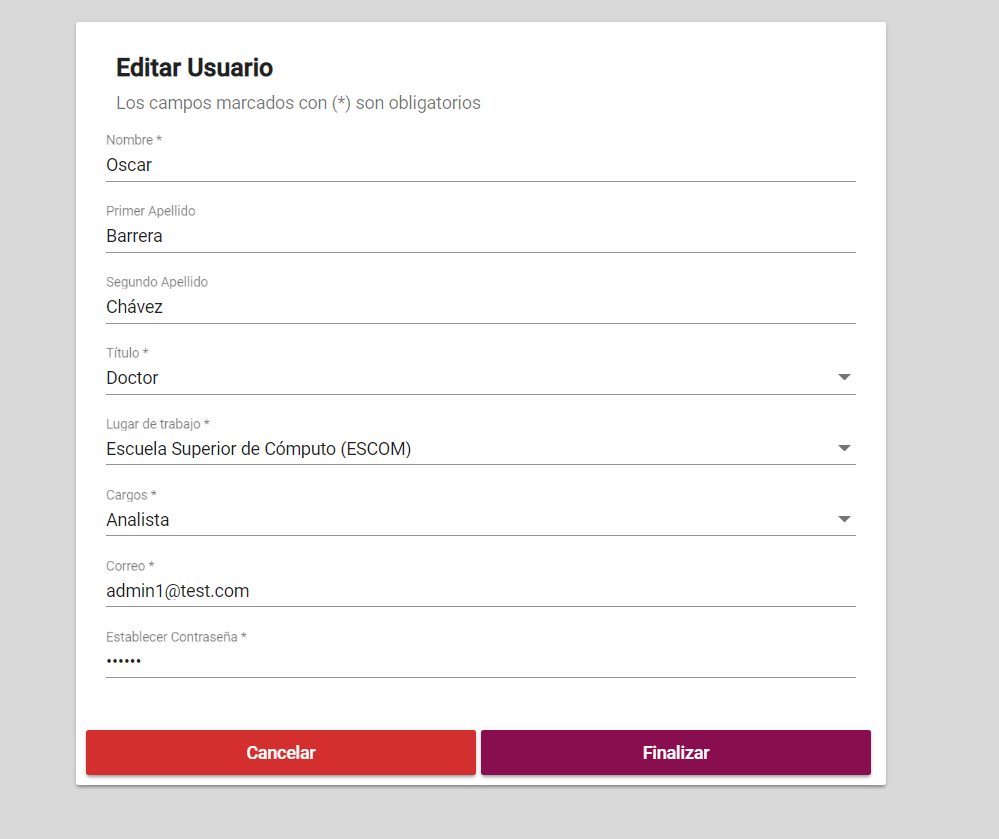
\includegraphics[width=0.6\linewidth]{images/SP5/Editar-Usuario}}
  	\caption{Pantalla para la edición de Usuarios}
  	\label{editarrh}
  \end{figure}

  En esta pantalla se cargarán los datos del usuario correspondiente por el lápiz amarillo seleccionado en la pantalla de \hyperlink{consultarUs}{\textit{Consultar Usuarios}} y llenará el formulario.

  A continuación, usted podrá modificar todos los campos del usuario.

  Si usted presiona el botón de “Cancelar”:

  \begin{figure}[H]
  	\centering
  	\hypertarget{cancel2}{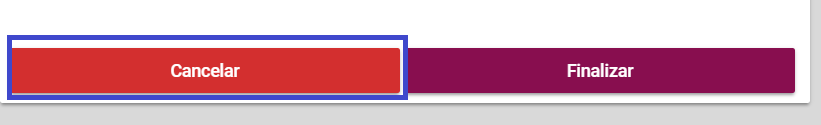
\includegraphics[width=0.7\linewidth]{images/SP5/BtnCancelar2}}
  	\caption{Botón ''Cancelar''}
  	\label{cancel2}
  \end{figure}

  El sistema mostrará el siguiente mensaje:
  %Imagen MSG29
  \clearpage
  \begin{figure}[H]
  	\centering
  	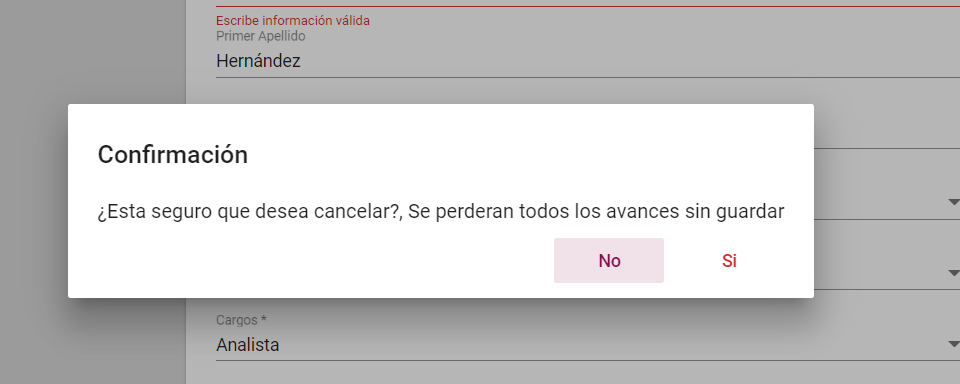
\includegraphics[width=0.4\linewidth]{images/SP5/MSG29}
  	\caption{Cancelar cambios}
  	\label{mensaje29}

  \end{figure}

  Para confirmar, usted tendrá que dar clic en el botón “Sí”, los datos del usuario no será modificados  y regresará a la pantalla \hyperlink{consultarUs}{\textit{Consultar Usuarios}}

  Para continuar con la modificación, usted tendrá que  dar clic el botón “No”, el mensaje se cerrará y usted continuará en el formulario para terminar la modificación.

  Cuando usted considere que los datos son correctos y están completos, deberá de dar clic en el botón “Finalizar”.
  \begin{figure}[H]
  	\centering
  	\hypertarget{btnfin}{
\includegraphics[width=0.7\linewidth]{images/SP5/BtnFinalizar}}
  	\caption{Botón ''Finalizar''}
  	\label{btnfin}
  \end{figure}

  Si no se presentan errores el sistema muestra el mensaje:
  %Imagen MSG31

  \begin{figure}[H]
  	\centering
  	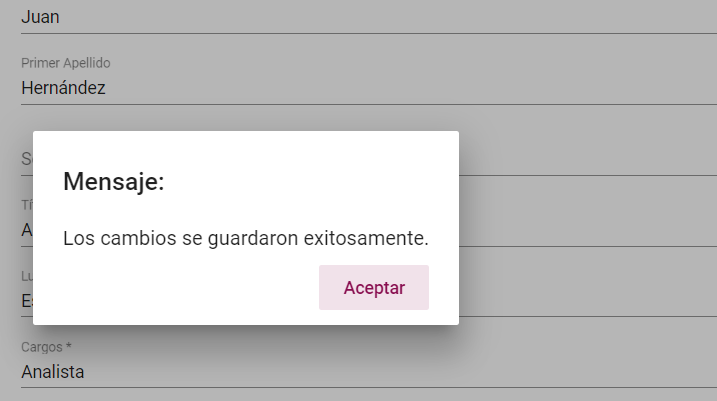
\includegraphics[width=0.4\linewidth]{images/SP5/MSG31}
  	\caption{Cambios guardados}
  	\label{mensaje31}

  \end{figure}

  Al dar clic en el botón “Aceptar”, el sistema mostrará la pantalla de \hyperlink{consultarUs}{\textit{Consultar Usuarios}}.

  \subsubsection{Posibles errores}
  \begin{itemize}
  	\item Problemas con la conexión o el sistema

  	Si al momento de acceder a la pantalla de \hyperlink{editarUs}{\textit{Editar Usuario}} o al intentar modificar un Usuario, aparece el siguiente mensaje:
  	\clearpage
  	\begin{figure}[H]
  		\centering
  		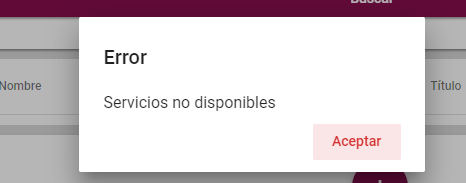
\includegraphics[width=0.4\linewidth]{images/SP5/MSGSN}
  		\caption{Servicios no disponibles}

  	\end{figure}


  	Significa que existió un error de conexión o del sistema. Al dar clic en en botón ''Aceptar'', el sistema lo redireccionará  a la pantalla de \hyperlink{consultarUs}{\textit{Consultar Usuarios}}. Deberá esperar a que la página este disponible para intentar acceder nuevamente.

  	\item Campos vacíos al momento de modificar al usuario

  	Si usted deja en blanco algún campo o campos del formulario, y posteriormente dio clic en el botón ''Finalizar'', el sistema mostrará el siguiente mensaje debajo del campo o campos:
  	%Imagen MSG3X

  	\begin{figure}[H]
  		\centering
  		
\includegraphics[width=0.4\linewidth]{images/SP5/MSG44}
  		\caption{Campos vacíos}
  		\label{mensaje44}

  	\end{figure}

  	Regresará  al formulario, en donde usted deberá llenar el o los campos que dejo vacíos.
  	\item El correo ingresado ya existe

  	Si al momento de dar clic en el botón ''Finalizar'' aparece el siguiente mensaje:
  	%Imagen MSG36

  	\begin{figure}[H]
  		\centering
  		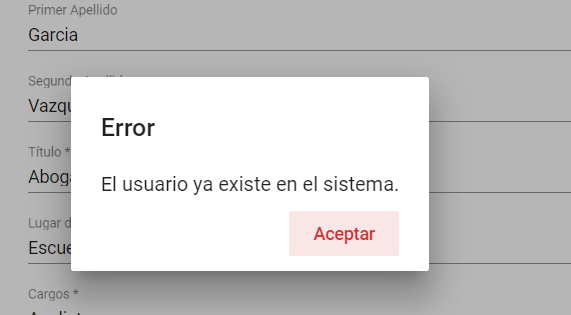
\includegraphics[width=0.4\linewidth]{images/SP5/MSG36}
  		\caption{El usuario ya existe}
  		\label{mensaje36}

  	\end{figure}

  	Significa que el Usuario ya se encuentra registrado en el sistema, por lo que éste impide que se vuelva a agregar nuevamente. Al dar clic en botón ''Aceptar'', el mensaje se cerrará y usted regresará al formulario. Aquí usted puede hacer dos acciones: verificar que el correo sea uno no registrado previamente e intentar agregar al Usuario nuevamente, o abandonar la pantalla de \hyperlink{registrarUs}{\textit{Registrar Usuarios}} e ir a otras partes del sistema.

  	\item Los campos ingresados no son válidos

  	Si al momento de dar clic en el botón ''Finalizar'' aparece el siguiente mensaje:
  	\clearpage
  	\begin{figure}[H]
  		\centering
  		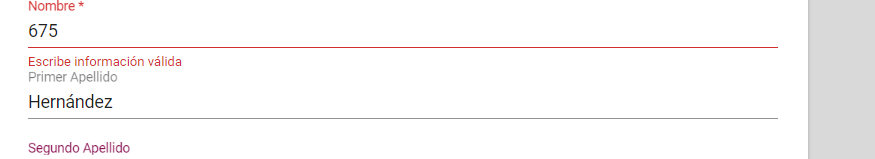
\includegraphics[width=0.4\linewidth]{images/SP5/MSG35}
  		\caption{Campos incorrectos}
  		\label{mensaje35}

  	\end{figure}


  	Significa que la composición de los datos ingresados en el formulario no es la correcta. Tenga en cuenta lo siguiente:

  	\begin{itemize}
  		\item El nombre y apellidos debe iniciar con mayúscula, puede poner más de uno por campo en caso de 2 nombres o apellidos compuestos.
  		\item Usted altero la información de los selectores de cargo o zona de trabajo.
  		\item La contraseña no acepta acentos, espacios o caracteres especiales.
  	\end{itemize}
\end{itemize}